\section{Lists Recap}
\label{sec:lists_recap}

\begin{frame}
	\frametitle{Doubly-Linked Lists}
		\begin{columns}
			\column{0.655\textwidth}
		\begin{center}
			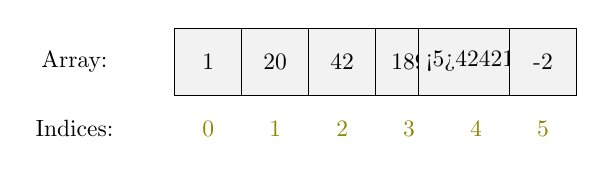
\begin{tikzpicture}[scale=0.85, transform shape]
	\foreach \x/\val in {0/1,1/20,2/42,3/189,4/\alt<5>{\alert{4242}}{17},5/-2}{
	\node[draw,rectangle, fill=gray!10, minimum size =1cm] (c) at (\x,0) {\val};
	\node[olive] (index) at (\x,-1) {\x};
}
\node[] at (-2,0) {Array:};
\node[] at (-2,-1) {Indices:};
\end{tikzpicture}

		\end{center}
			\column{0.355\textwidth}
			\begin{block}{An array}
				A block of memory, index-based.
			\end{block}	
		\end{columns}
		\pause
		\begin{columns}
			\column{0.655\textwidth}
		\begin{center}
			% Tikz template taken from: https://tex.stackexchange.com/a/19288
\begin{tikzpicture}[list/.style={rectangle split, rectangle split parts=2,
    draw, rectangle split horizontal}, >=stealth, start chain]

  \node[list,on chain] (A) {42};
  \node[list,on chain] (B) {99};
  \draw[*->] let \p1 = (A.two), \p2 = (A.center) in (\x1,\y2) -- (B);
  \node[list,on chain] (C) {12};
  \draw[*->] let \p1 = (B.two), \p2 = (B.center) in (\x1,\y2) -- (C);
  \node[on chain,draw,inner sep=6pt] (D) {};
  \draw (D.north east) -- (D.south west);
  \draw (D.north west) -- (D.south east);
  \draw[*->] let \p1 = (C.two), \p2 = (C.center) in (\x1,\y2) -- (D);

\end{tikzpicture}	

		\end{center}
			\column{0.355\textwidth}
			\begin{block}{A singly linked list}
				Only has connections in one direction.	
			\end{block}	
		\end{columns}
		\pause
		\begin{columns}
			\column{0.655\textwidth}
				
			\begin{center}
				% Tikz template taken from: https://tex.stackexchange.com/a/19288
\begin{tikzpicture}[list/.style={rectangle split, rectangle split parts=2,
    draw, rectangle split horizontal},start chain]

		\only<2->{
  \node[on chain,draw,inner sep=6pt] (E) {};
  \draw (E.north east) -- (E.south west);
  \draw (E.north west) -- (E.south east);
}
  \node[list,on chain] (A) {42};
  \node[list,on chain] (B) {99};
  \draw[*->] let \p1 = (A.two), \p2 = (A.center) in (\x1,\y2) -- (B);
  \node[list,on chain] (C) {12};
  \draw[*->] let \p1 = (B.two), \p2 = (B.center) in (\x1,\y2) -- (C);
  \node[on chain,draw,inner sep=6pt] (D) {};
  \draw (D.north east) -- (D.south west);
  \draw (D.north west) -- (D.south east);
  \draw[*->] let \p1 = (C.two), \p2 = (C.center) in (\x1,\y2) -- (D);

	\only<2->{
		\draw[->,red,thick] let \p1 = (A.two), \p2 = (A.center) in (B) to [out=150, in=30] (\x1,\y2);
		\draw[->,red,thick] let \p1 = (B.two), \p2 = (B.center) in (C) to [out=150, in=30] (\x1,\y2);
		\draw[->,red,thick] let \p1 = (E.center), \p2 = (E.center) in (A) to [out=150, in=30] (\x1,\y2);
	}
\end{tikzpicture}	

			\end{center}
			\column{0.355\textwidth}
			\begin{block}{A doubly linked list}
				Has connections in both directions.
			\end{block}
				
		\end{columns}
\end{frame}

\begin{frame}
	\frametitle{Remember lists?}
	
	\begin{tabular}{l | c | c | c}
	Operation & Array-based list & SLL & DLL \\	
	\midrule
	Get element $k$ & $O(1)$ &$O(k)$ & $O(k)$ \\
	Insert first element& $O(n)$ & $O(1)$ & $O(1)$\\
	Insert at index $k$& $O(n-k)$ & $O(k)$ & $O(\min(k,n-k))$\\
	Append (amortised)& $O(1)$ & $O(1)$ & $O(1)$\\
	Remove first element& $O(n)$ & $O(1)$ & $O(1)$\\
	Remove last element& $O(1)$ & $O(n)$ & $O(1)$\\
	Remove index $k$& $O(n-k)$ & $O(k)$ & $O(\min(k,n-k))$\\
	Search & $O(n)$ & $O(n)$ & $O(n)$\\
	\end{tabular}

\end{frame}
